\documentclass[epsfig,10pt,fullpage]{article}

\newcommand{\LabNum}{2}
\newcommand{\CommonDocsPath}{../../../common/docs}
\addtolength{\textwidth}{1.5in}
\addtolength{\oddsidemargin}{-0.75in}
\addtolength{\topmargin}{-0.75in}
\addtolength{\textheight}{1.5in}
\addtolength{\evensidemargin}{0.75in}
\setlength\parindent{0pt}
\raggedbottom

\usepackage{ae,aecompl}
\usepackage{epsfig,float,times}
\usepackage[hypcap]{caption}
\usepackage[pdftex, colorlinks]{hyperref}
\usepackage{graphicx}
\usepackage[usenames, dvipsnames]{color}
\usepackage{rotating}
\usepackage{tikz}
\usetikzlibrary{automata,positioning}
\usepackage{placeins}

\widowpenalty 10000
\clubpenalty 10000

\newcommand{\red}[1]{{\color{red}\sf{#1}}}
\newcommand{\green}[1]{{\color{green}\sf{#1}}}
\newcommand{\blue}[1]{{\color{blue}\sf{#1}}}
\definecolor{PineGreen}{rgb}{0.0, 0.47, 0.44}
\definecolor{ForestGreen}{rgb}{0.13, 0.55, 0.13}
\definecolor{Brown}{rgb}{0.59, 0.29, 0.0}

\newcommand{\UPDatePublished}{Oct 2021}
\newcommand{\versnum}{21.1} %version number quartus/AMP
\newcommand{\quartusname}{Quartus\textsuperscript{\textregistered} Prime}	
\newcommand{\UPTextBar}{For \quartusname{} \versnum{}}
\newcommand{\thisyear}{2021 } %for copyright
\newcommand{\company}{FPGAcademy.org}
\newcommand{\longteamname}{FPGAcademy.org}
\newcommand{\teamname}{FPGAcademy}
\newcommand{\website}{FPGAcademy.org}

\newcommand{\productAcronym}{AMP}
\newcommand{\productNameShort}{Monitor Program}

\newcommand{\productNameMedTM}{A Monitor Program}
\newcommand{\productNameMed}{A Monitor Program}

%\newcommand{\headerLogoFilePath}[1]{#1/FPGAcademy.png}

% listings is a package that supports encapsulating source code in LaTeX conveniently
\usepackage{listings}

\def\expandparam\lstinputlisting[#1]#2{\edef\tmp{\noexpand\lstinputlisting[#1]{#2}}\tmp}

%%%%%%%%%%%%%%%%%%%% Source Code Formatting %%%%%%%%%%%%%%%%%%%%
\definecolor{globalCommentColour}{rgb}{0.588,0.588,0.588}

%%%%%%%%%%%%%%%%%%%%%%%%%%%%%%%%%%%%%%%%%%%%%%%%%%%%
% Defining language style
% NiosII ASM
\lstdefinelanguage[NiosII]{Assembler} {
  morekeywords={add, addi, and, andhi, andi, beq, bge, bgeu, bgt, bgtu, ble,  bleu, blt, bltu, bne, br, break,
  bret, call, callr, cmpeq, cmpeqi, cmpge, cmpgei, cmpgeu, cmpgeui, cmpgt, cmpgti, cmpgtu, cmpgtui, cmple,
  cmplei, cmpleu, cmpleui, cmplt, cmplti, cmpltu, cmpltui, cmpne, cmpnei, custom, div, divu, eret, flushd,
  flushda, flushi, flushp, initd, initda, initi, jmp, jmpi, ldb, ldbio, ldbu, ldbuio, ldh, ldhio, ldhu, ldhuio,
  ldw, ldwio, mov, movhi, movi, movia, movui, mul, muli, mulxss, mulxsu, mulxuu, nextpc, nop, nor, or, orhi, ori,
  rdctl, rdprs, ret, rol, roli, ror, sll, slli, sra, srai, srl, srli, stb, stbio, sth, sthio, stw, stwio,
  sub, subi, sync, trap, wrctl, wrtcl, wrprs, xor, xori, xorhi, xori},
  morekeywords=[2]{.abort, .ABORT, .align, .app-file, .ascii, .asciz, .balign, .byte, .comm, .data, .def,
  .desc, .dim, .double, .eject, .else, .end, .endef, .endif, .equ, .equiv, .err, .extern, .file, .fill, .float,
  .global, .globl, .hword, .ident, .if, .include, .int, .irp, .irpc, .lcomm, .lflags, .line, .linkonce, .ln,
  .list, .long, .macro, .mri, .nolist, .octa, .org, .p2align, .psize, .quad, .rept, .sbttl, .scl, .section,
  .set, .short, .single, .size, .sleb128, .skip, .space, .stadb, .stabn, .stabs, .string, .symver, .tag,
  .text, .title, .type, .val, .uleb128, .word},
  morekeywords=[3]{et, bt, gp, sp, fp, ea, sstatus, ra, pc, status, estatus, bstatus, ienable, ipending, cpuid,
  exception, pteaddr, tlbacc, tlbmisc, eccinj, badaddr, config, mpubase, mpuacc},
  sensitive=t,
  alsoletter=.,
  morestring=[b]",
  morecomment=[s]{/*}{*/},
  morecomment=[l]\#,
}[keywords,comments,strings]
   
%% NOTE: morekeywords=[2] are GNU directives.
   
\definecolor{niosInstructionColour}{rgb}{0.000,0.608,0.000}
\definecolor{niosDirectiveColour}{rgb}{0.000,0.000,0.902}
\definecolor{niosSpecialRegColour}{rgb}{0.000,0.000,0.000}
\definecolor{niosStringColour}{rgb}{0.808,0.482,0.000}
   
%% NOTE: To make bold use: =\bfseries\color{<colour>}
\lstdefinestyle{defaultNiosStyle} {
  language=[NiosII]{Assembler},
  stringstyle=\color{niosStringColour},
  keywordstyle=\color{niosInstructionColour},
  keywordstyle=[2]\color{niosDirectiveColour},
  keywordstyle=[3]\itshape\color{niosSpecialRegColour}
}
%%%%%%%%%%%%%%%%%%%%%%%%%%%%%%%%%%%%%%%%%%%%%%%%%%%%

%%%%%%%%%%%%%%%%%%%%%%%%%%%%%%%%%%%%%%%%%%%%%%%%%%%%
% Defining language style
% ArmA9 ASM
\lstdefinelanguage[ArmA9]{Assembler} {
  morekeywords={ADC, ADD, ADDS, AND, ANDS, B, BAL, BEQ, BGE, BGT, BL, BLT, BIC, BKPT, BLX, BNE, BX, CDP, CLZ, CMN, CMP, EOR,
  EORS, LDC, LDM, LDR, LDRB, LDRBT, LDRH, LDRSB, LDRSH, LDRT, LSL, MCR, MLA, MOV, MOVW, MOVT, MRC, MRS, MSR, MUL, MVN, ORR, PLD,
  ROR, RSB, RSC, SBC, SMLAL, SMULL, STC, STM, STR, STRB, STRBT, STRH, STRT, SUB, SUBS, SWI, SWP, SWPB, TEQ, UMLAL,
  PUSH, POP, MOVS, RORS, LSR},
  morekeywords=[2]{.abort, .ABORT, .align, .app-file, .ascii, .asciz, .balign, .byte, .comm, .data, .def,
  .desc, .dim, .double, .eject, .else, .end, .endef, .endif, .equ, .equiv, .err, .extern, .file, .fill, .float,
  .global, .globl, .hword, .ident, .if, .include, .int, .irp, .irpc, .lcomm, .lflags, .line, .linkonce, .ln,
  .list, .long, .macro, .mri, .nolist, .octa, .org, .p2align, .psize, .quad, .rept, .sbttl, .scl, .section,
  .set, .short, .single, .size, .sleb128, .skip, .space, .stadb, .stabn, .stabs, .string, .symver, .tag,
  .text, .title, .type, .val, .vectors, .uleb128, .word},
  morekeywords=[3]{SP, PC, MIDR, CTR, TCMTR, TLBTR, MPIDR, ID_PFR0, ID_PFR1, ID_DFR0, ID_MMFR0, ID_MMFR1, ID_MMFR2,
  ID_MMFR3, ID_ISAR0, ID_ISAR1, ID_ISAR2, ID_ISAR3, ID_ISAR4, CCSIDR, CLIDR, AIDR, CSSELR, TTBR0, TTRB1, TTBR2, DACR,
  DFSR, IFSR, ADFSR, AIFSR, DFAAR, IFAR, ICIALLUIS, BPIALLIS, PAR, ICIALLU, ICIMVAU, BPIALL, DCIMVAC, DCISW, V2PCWPR,
  DCCVAC, DCCSW, DDIMVAC, DCISW, TLBALLIS, TLBIMVAIS, TLBIASIDIS, TLBIMVAAIS, TLBIALL, TLBIMVA, TLBIASID, TLBIMVAA,
  PMCR, PMCNTENSET, PMCNTENCLR, PMOVSR, PMSWINC, PMSELR, PMXEVTYPER, PMXEVCNTR, PMUSERENR, PMINTENSET, PMINTENCLR,
  PRRR, NRRR, PLEIDR, PLEASR, PLEFSR, PLEUAR, PLEPCR, VBAR, MVBAR, ISR, FCSEIDR, CONTEXTIDR, TPIDRURW, TPIDRURO, TPIDRPRW},
  sensitive=f,
  alsoletter=.,
  morestring=[b]",
  morecomment=[s]{/*}{*/},
  morecomment=[l]{//},
}[keywords,comments,strings]
   
%% NOTE: morekeywords=[2] are GNU directives.
   
\definecolor{armInstructionColour}{rgb}{0.000,0.608,0.000}
\definecolor{armDirectiveColour}{rgb}{0.000,0.000,0.902}
\definecolor{armSpecialRegColour}{rgb}{0.000,0.000,0.000}
\definecolor{armStringColour}{rgb}{0.808,0.482,0.000}
   
\lstdefinestyle{defaultArmStyle} {
  language=[ArmA9]{Assembler},
  stringstyle=\color{armStringColour},
  keywordstyle=\color{armInstructionColour},
  keywordstyle=[2]\color{armDirectiveColour},
  keywordstyle=[3]\itshape\color{armSpecialRegColour}
}
%%%%%%%%%%%%%%%%%%%%%%%%%%%%%%%%%%%%%%%%%%%%%%%%%%%%

%%%%%%%%%%%%%%%%%%%%%%%%%%%%%%%%%%%%%%%%%%%%%%%%%%%%
% Defining language style
% FPGAcademy ASM
\lstdefinelanguage{ASM}{
  morekeywords = [1]{mv, mvt, mvne, mvcc, add, sub, st, ld, and, b, bne, beq, bcc, bcs},
  morekeywords = [2]{word, define},
  keywordstyle = [1]\color{ForestGreen},
  keywordstyle = [2]\color{blue},
  sensitive = true,
  morecomment = [l]{//},
}

\lstset{
  language = ASM,
  basicstyle=\small\color{black}\ttfamily,
  commentstyle=\small\color{Brown}\itshape\ttfamily,
  showstringspaces=false,
  frame=none, %lines % boxed listings
  breaklines=true,
  breakatwhitespace=true,
  tabsize=3
}
%%%%%%%%%%%%%%%%%%%%%%%%%%%%%%%%%%%%%%%%%%%%%%%%%%%%

%%%%%%%%%%%%%%%%%%%%%%%%%%%%%%%%%%%%%%%%%%%%%%%%%%%%
% Defining language style
% Java
\definecolor{javaStringColour}{rgb}{0.808,0.482,0}
%%%%%%%%%%%%%%%%%%%%%%%%%%%%%%%%%%%%%%%%%%%%%%%%%%%%

%%%%%%%%%%%%%%%%%%%%%%%%%%%%%%%%%%%%%%%%%%%%%%%%%%%%
% Defining language style
% C
\definecolor{CStringColour}{rgb}{0.808,0.482,0}

\lstset{
  language = C,
  basicstyle=\small\color{black}\ttfamily, 
  commentstyle=\small\color{PineGreen}\itshape\ttfamily,
  keywordstyle=\small\color{blue}\bfseries\ttfamily,
  showstringspaces=false,
  frame=none, %lines % boxed listings
  breaklines=true,
  breakatwhitespace=true,
  tabsize=3
}
%%%%%%%%%%%%%%%%%%%%%%%%%%%%%%%%%%%%%%%%%%%%%%%%%%%%

%%%%%%%%%%%%%%%%%%%%%%%%%%%%%%%%%%%%%%%%%%%%%%%%%%%%
% Defining language style
% Verilog
\definecolor{verilogCommentColour}{rgb}{0.000,0.502,0.000}

\lstdefinestyle{defaultVerilogStyle} {
  language={Verilog},
  keywordstyle=\color{blue},
  commentstyle=\color{verilogCommentColour}
}
%%%%%%%%%%%%%%%%%%%%%%%%%%%%%%%%%%%%%%%%%%%%%%%%%%%%

%%%%%%%%%%%%%%%%%%%%%%%%%%%%%%%%%%%%%%%%%%%%%%%%%%%%
% Defining language style
% VHDL
\lstdefinestyle{defaultVHDLStyle} {
  language={VHDL},
  keywordstyle=\color{blue},
  commentstyle=\color{verilogCommentColour}
}
%%%%%%%%%%%%%%%%%%%%%%%%%%%%%%%%%%%%%%%%%%%%%%%%%%%%

%%%%%%%%%%%%%%%%%%%%%%%%%%%%%%%%%%%%%%%%%%%%%%%%%%%%
% Defining language style
% LaTeX
\lstdefinelanguage[LocalLaTeX]{TeX}[LaTeX]{TeX}{moretexcs={bf, it, sf, lstset},}

\lstdefinestyle{defaultLocalLatexStyle} {
  language=[LocalLatex]{TeX},
  keywordstyle=\color{blue}\bfseries,
  keywordstyle=[2]\color{blue},
  keywordstyle=[3]\color{blue}\bfseries
}
%%%%%%%%%%%%%%%%%%%%%%%%%%%%%%%%%%%%%%%%%%%%%%%%%%%%

%%%%%%%%%%%%%%%%%%%%%%%%%%%%%%%%%%%%%%%%%%%%%%%%%%%%
% Defining language style
% Default
\lstset{
  basicstyle=\small\color{black}\ttfamily,
  commentstyle=\small\color{globalCommentColour}\itshape\ttfamily,
  keywordstyle=\small\color{blue}\bfseries\ttfamily,
  showstringspaces=false,
  frame=none, %lines % boxed listings
  breaklines=true,
  breakatwhitespace=true,
  tabsize=3
}
%%%%%%%%%%%%%%%%%%%%%%%%%%%%%%%%%%%%%%%%%%%%%%%%%%%%


\hypersetup{
  pdftitle={Digital Logic Lab Exercise \LabNum},
  linkcolor=blue,
  hyperindex=true,
  pdfauthor={FPGAcademy.org},
  pdfkeywords={FPGAcademy.org, FPGAcademy, Lab, Exercise, Digital Logic},
  bookmarks,
  bookmarksopen=false,
  filecolor=blue,
  pdfstartview={FitH},
  urlcolor=blue,
  plainpages=false,
  pdfpagelabels=true,
  linkbordercolor={1 1 1} %no color for link border
}



\begin{document}

\centerline{\huge Digital Logic}
~\\
\centerline{\huge Laboratory Exercise \LabNum}
~\\
\centerline{\large Numbers and Displays}
~\\

\noindent
This is an exercise in designing combinational circuits that can perform
binary-to-decimal number conversions and binary-coded-decimal (BCD) addition.
~\\

\section*{Part I}
\addcontentsline{toc}{1}{Part I}
We wish to display on the 7-segment displays {\it HEX1} and {\it HEX0} the 
values set by the switches $SW_{7-0}$. 
Let the values denoted by $SW_{7-4}$ and $SW_{3-0}$ be displayed on {\it HEX1} and {\it HEX0}, 
respectively.
Your circuit should be able to display the digits from 0 to 9, and should treat the
valuations 1010 to 1111 as don't-cares.

\begin{enumerate}
\item Create a new project which will be used to implement the desired
circuit on your Intel\textsuperscript{\textregistered} FPGA DE-series board. The intent of this exercise is to manually 
derive the logic functions needed for the 7-segment displays. Therefore, you should use only
simple VHDL assignment statements in your code and specify each logic function as
a Boolean expression.
\item Write a VHDL file that provides the necessary functionality. Include this 
file in your project and assign the pins on the FPGA to connect to the 
switches and 7-segment displays. Make sure to include the necessary pin assignments.
\item Compile the project, generate a .qsf file in Quartus and upload it to the NO-IDE lab of LabsLand.
\item Test the functionality of your design by toggling the switches
and observing the displays.
\item For more info, if you have a FPGA chip, you can download the compiled circuit into the FPGA chip.
\end{enumerate}

\section*{Part II}
\addcontentsline{toc}{2}{Part II}
You are to design a circuit that converts a four-bit binary number $V = v_3 v_2 v_1 v_0$
into its two-digit decimal equivalent $D = d_1 d_0$. Table~\ref{tab:BtD} shows the required output
values. A partial design of this circuit is given in Figure \ref{fig:fig1}. It includes a comparator
that checks when the value of $V$ is greater than 9, and uses the output of this
comparator in the control of the 7-segment displays. You are to complete the design of
this circuit. 

\begin{table}[H]
\begin{center}
\begin{tabular}{c|c c}
$v_3 v_2 v_1 v_0$& $d_1$&$d_0$\\ \hline
\hspace{0.75 mm} {\rule[0mm]{0mm}{5mm}0000} & 0 & 0\\ 
\hspace{0.75 mm} 0001 & 0 & 1\\
\hspace{0.75 mm} 0010 & 0 & 2\\
\hspace{0.75 mm} {\rule[0mm]{0mm}{2.5mm}$\ldots$} & $\ldots$ & $\ldots$ \\
\hspace{0.75 mm} {\rule[0mm]{0mm}{5mm}1001} & 0 & 9\\
\hspace{0.75 mm} 1010 & 1 & 0\\
\hspace{0.75 mm} 1011 & 1 & 1\\
\hspace{0.75 mm} 1100 & 1 & 2\\
\hspace{0.75 mm} 1101 & 1 & 3\\
\hspace{0.75 mm} 1110 & 1 & 4\\
\hspace{0.75 mm} 1111 & 1 & 5\\
\end{tabular}
	\caption{Binary-to-decimal conversion values.}
	\label{tab:BtD}
\end{center}
\end{table}

The output $z$ for the comparator circuit can be specified using a 
single Boolean expression, with the four inputs $V_{3-0}$. 
Design this Boolean expression by making a truth table that shows the valuations of 
the inputs $V_{3-0}$ for which $z$ has to be 1. 

\begin{figure}[H]
	\begin{center}
		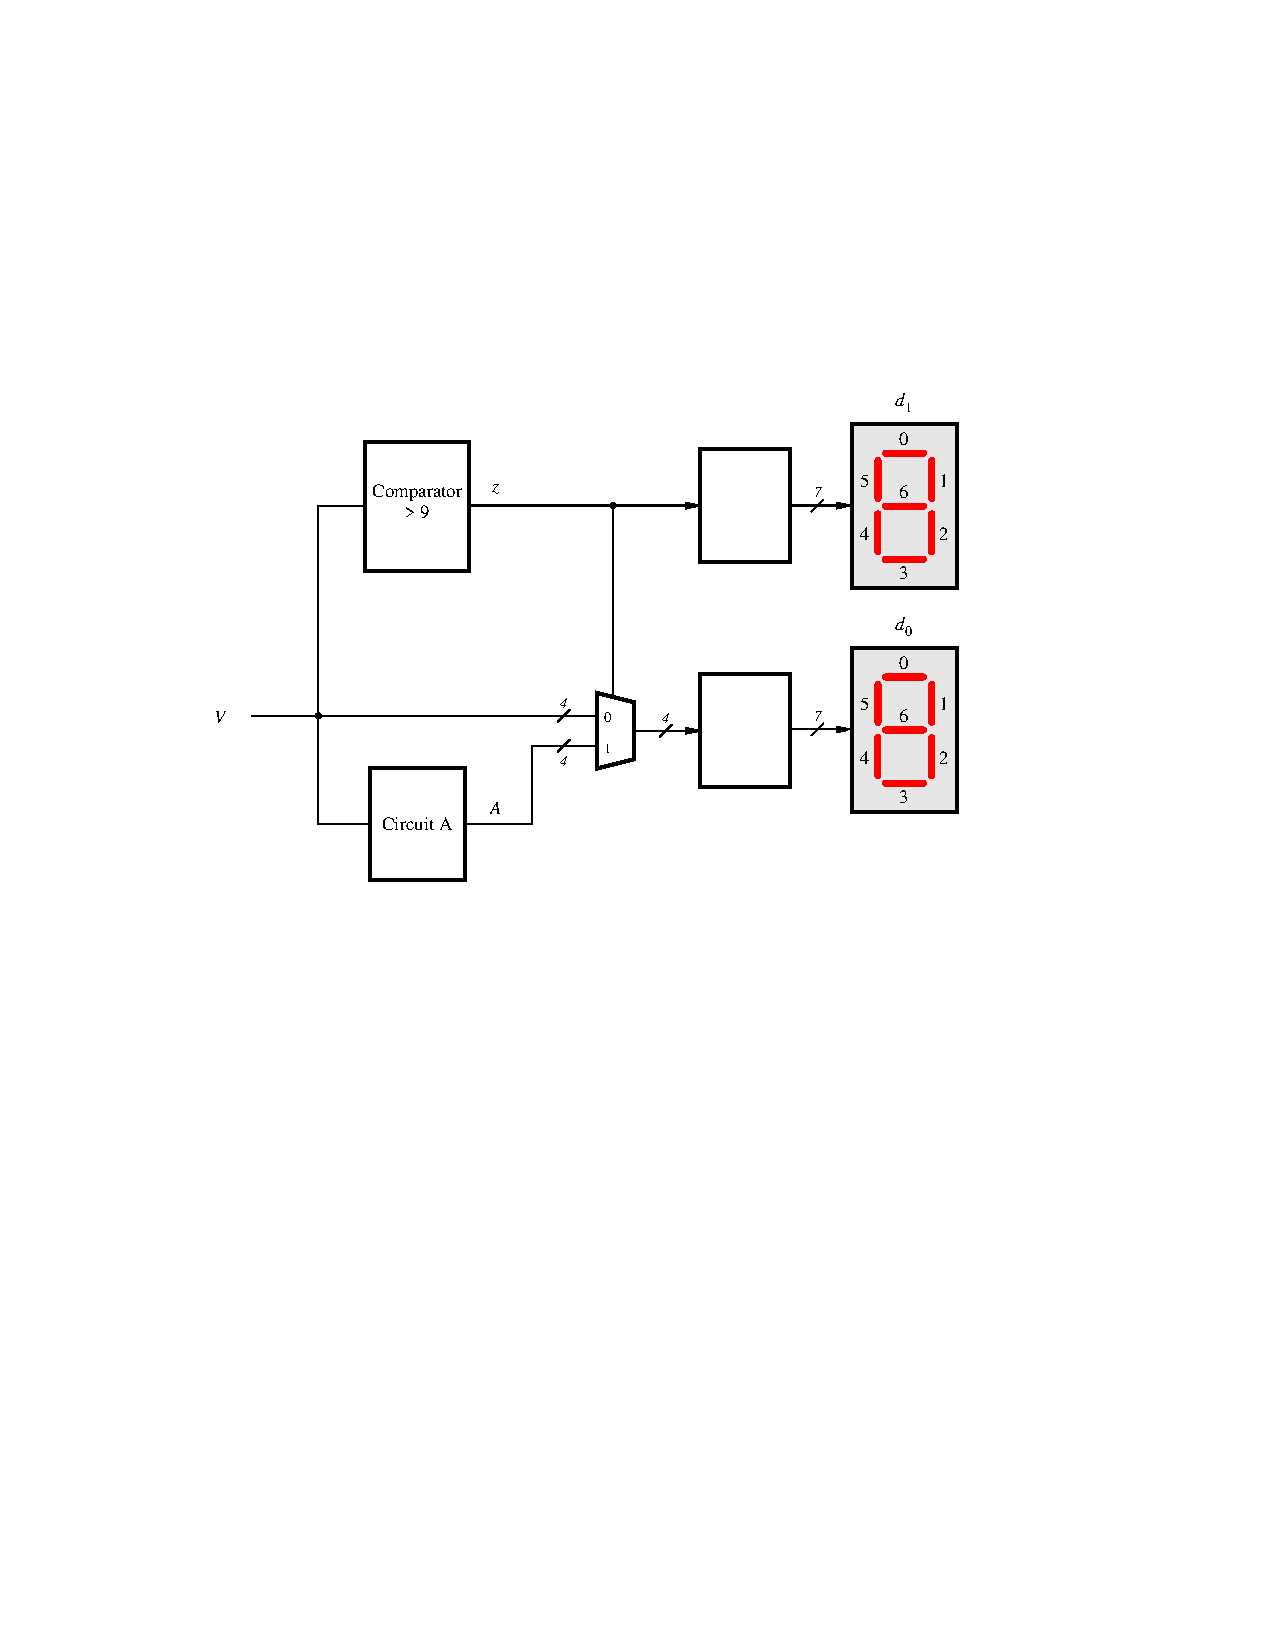
\includegraphics[]{figures/figure1.pdf}
	\end{center}
\caption{Partial design of the binary-to-decimal conversion circuit.}
\label{fig:fig1}
\end{figure}

Notice that the circuit in Figure~\ref{fig:fig1} includes a 4-bit wide 2-to-1 multiplexer (a similar multiplexer
was described as part of Laboratory Exercise 1). The purpose of this multiplexer is to 
drive digit $d_0$ with the value of $V$ when $z=0$, and the value of $A$ when $z=1$.
To design circuit $A$ consider the following. For the input values $V \le 9$, the circuit $A$
does not matter, because the multiplexer in Figure \ref{fig:fig1} just selects $V$ in
these cases. But for the input values $V > 9$, the multiplexer will select $A$.
Thus, $A$ has to provide output values that properly implement 
Table~\ref{tab:BtD} when $V > 9$.  You need to design circuit $A$ so that the input $V = 1010$ gives 
an output $A = 0000$, the input $V = 1011$ gives the output $A = 0001$, $\ldots$, and the 
input $V = 1111$ gives the output $A = 0101$.  Design circuit $A$ by making a truth table with 
the inputs $V_{3-0}$ and the outputs $A_{3-0}$.

~\\
Perform the following steps:

\begin{enumerate}
\item Write VHDL code to implement your design. The code
should have the 4-bit input $SW_{3-0}$, which should be
used to provide the binary number $V$, and the two 7-bit outputs {\it HEX1} and {\it HEX0},
to show the values of decimal digits $d_1$ and $d_0$. 
The intent of this exercise is to use simple VHDL assignment
statements to specify the required logic functions using Boolean
expressions. Your VHDL code should not include any IF-ELSE, CASE, or
similar statements. 
\item Make a Quartus\textsuperscript{\textregistered} project for your VHDL entity.
\item Compile the circuit and use functional simulation to verify the correct operation of
your comparator, multiplexers, and circuit {\it A}.
\item Generate a .qsf file in Quartus and upload it to the NO-IDE lab of LabsLand. Test the circuit by trying all possible
values of $V$ and observing the output displays.
\item For more info, if you have a FPGA chip, you can download the compiled circuit into the FPGA chip.
\end{enumerate}

\section*{Part III}
\addcontentsline{toc}{3}{Part III}
Figure \ref{fig:fig2}$a$ shows a circuit for a {\it full adder}, 
which has the inputs $a$, $b$, and $c_i$,
and produces the outputs $s$ and $c_o$. Parts $b$ and $c$ of the figure show a circuit
symbol and truth table for the full adder, which produces the two-bit binary sum
$c_o s = a + b + c_i$. Figure \ref{fig:fig2}$d$ shows how four instances of this full adder module
can be used to design a circuit that adds two four-bit numbers. This type of circuit is
usually called a {\it ripple-carry} adder, because of the way that the carry signals are 
passed from one full adder to the next. Write VHDL code that implements this circuit,
as described below.

\begin{figure}[H]
	\begin{center}
		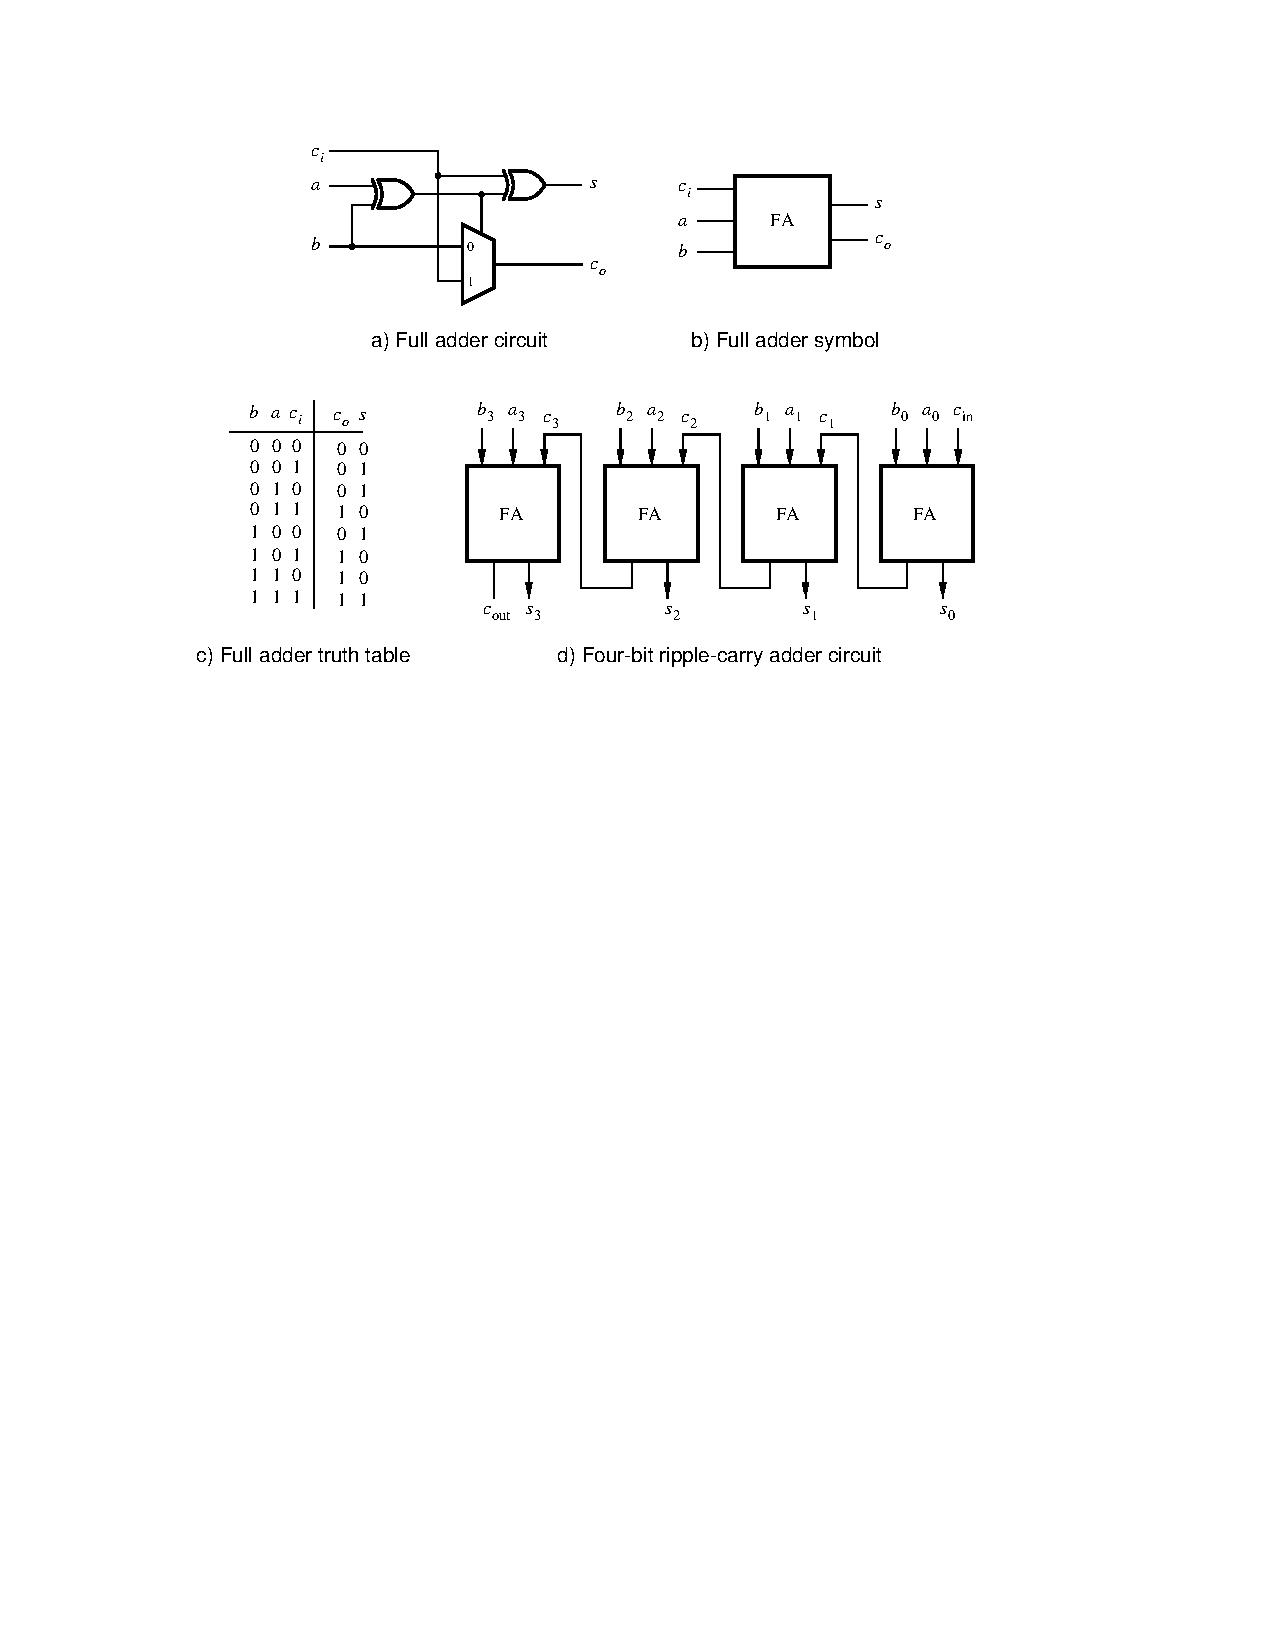
\includegraphics[]{figures/figure2.pdf}
	\end{center}
\caption{A ripple-carry adder circuit.}
\label{fig:fig2}
\end{figure}

\begin{enumerate}
\item Create a new Quartus project for the adder circuit. Write a VHDL entity
for the full adder subcircuit and write a top-level VHDL entity that instantiates four 
instances of this full adder.
\item Use switches $SW_{7-4}$ and $SW_{3-0}$ to represent the inputs $A$ and $B$, respectively.
Use $SW_{8}$ for the carry-in $c_{in}$ of the adder. Connect the outputs of the adder, 
$c_{out}$ and $S$, to the red lights LEDR.
\item Include the necessary pin assignments for your DE-series board, compile the circuit, generate a .qsf file in Quartus and upload it to the NO-IDE lab of LabsLand.
\item Test your circuit by trying different values for numbers $A$, $B$, and $c_{in}$.
\item For more info, if you have a FPGA chip, you can download the compiled circuit into the FPGA chip.
\end{enumerate}

\section*{Part IV}
\addcontentsline{toc}{4}{Part IV}
In Part II we discussed the conversion of binary numbers into decimal digits. For this
part you are to design a circuit that has two decimal digits, $X$ and $Y$, as inputs.
Each decimal digit is represented as a 4-bit number. In technical literature this is 
referred to as the {\it binary coded decimal} (BCD) representation. 

You are to design a circuit that adds the two BCD digits. The inputs to your circuit
are the numbers $X$ and $Y$, plus a carry-in, $c_{in}$. When these inputs are
added, the result will be a 5-bit binary number. But this result is to be displayed
on 7-segment displays as a two-digit BCD sum $S_1 S_0$. For a sum equal to zero you
would display $S_1 S_0 = 00$, for a sum of one $S_1 S_0 = 01$, for nine 
$S_1 S_0 = 09$, for ten $S_1 S_0 = 10$, and so on. Note that the inputs 
$X$ and $Y$ are assumed to be decimal
digits, which means that the largest sum that needs to be handled by this 
circuit is $S_1 S_0 = 9 + 9 + 1 = 19$. 

Perform the steps given below.

\begin{enumerate}
\item Create a new Quartus project for your BCD adder. You should use the
four-bit adder circuit from Part III to produce a four-bit sum and carry-out for the
operation $X$ + $Y$. 

A good way to work out the design of your circuit is to first make it handle only sums
$(X + Y) \le 15$. With these values, your circuit from Part II can be used to convert the
4-bit sum into the two decimal digits $S_1 S_0$.  Then, once this is working, modify 
your design to handle values of $15 < (X + Y) \le 19$. One way to do this is to still use 
your circuit from Part II, but to modify its outputs before attaching them to the 7-segment 
display to make the necessary adjustments when the sum from the adder exceeds 15.

Write your VHDL code using
simple assignment statements to specify the required logic functions--do not use 
other types of VHDL
statements such as IF-ELSE or CASE statements for this part of the exercise.
\item Use switches $SW_{7-4}$ and $SW_{3-0}$ for the inputs $X$ and $Y$, respectively, and
use $SW_{8}$ for the carry-in. Connect the four-bit sum and carry-out produced 
by the operation $X$ + $Y$ to the red lights LEDR. Display the BCD values of $X$
and $Y$ on the 7-segment displays {\it HEX5} and {\it HEX3}, and display the result $S_1 S_0$ on
{\it HEX1} and {\it HEX0}.
\item Since your circuit handles only BCD digits, check for the cases when the input 
$X$ or $Y$ is greater than nine. If this occurs, indicate an error by turning on 
the red light {\it LEDR}$_9$.
\item Include the necessary pin assignments for your DE-series board, compile the circuit, generate a .qsf file in Quartus and upload it to the NO-IDE lab of LabsLand.
\item Test your circuit by trying different values for numbers $X$, $Y$, and $c_{in}$.
\item For more info, if you have a FPGA chip, you can download the compiled circuit into the FPGA chip.
\end{enumerate}

\section*{Part V}
\addcontentsline{toc}{5}{Part V}
In Part IV you created VHDL code for a BCD adder. A different approach for describing
the adder in VHDL code is to specify an algorithm like the one
represented by the following pseudo-code:

~\\
\begin{center}
\begin{minipage}[t]{12.5 cm}
\begin{tabbing}
ZZZ\=ZZ\=ZZ\=ZZ\=ZZ\=ZZ\=ZZ\=ZZ\=ZZ\=ZZ\=ZZ\kill
1\>$T_0 = A + B + c_0$ \\
2\>{\bf if} ($T_0 > 9$) {\bf then}\\
3\>\>$Z_0 = 10$;\\
4\>\>$c_1 = 1$;\\
5\>{\bf else}\\
6\>\>$Z_0 = 0$;\\
7\>\>$c_1 = 0$;\\
8\>{\bf end if}\\
9\>$S_0 = T_0 - Z_0$\\
10\>$S_1 = c_1$\\
\end{tabbing}
\end{minipage}
\end{center}
~\\
It is reasonably straightforward to see what circuit could be used to implement this
pseudo-code. Lines 1 and 9 represent adders, lines 2-8 correspond to
multiplexers, and testing for the condition $T_0 > 9$ requires comparators.
You are to write VHDL code that corresponds to this pseudo-code. Note that you can
perform addition operations in your VHDL code instead of the subtraction shown 
in line 9. The intent of this part of the exercise is
to examine the effects of relying more on the VHDL compiler to design the circuit by using
IF-ELSE statements along with the VHDL $>$ and $+$ operators. 
Perform the following steps:

\begin{enumerate}
\item Create a new Quartus project for your VHDL code. Use switches $SW_{7-4}$ and $SW_{3-0}$ for the inputs $A$ and $B$, respectively, and
use $SW_{8}$ for the carry-in.
The value of $A$ should be displayed on the 7-segment display {\it HEX5}, 
while $B$ should be on {\it HEX3}.
Display the BCD sum, $S_1 S_0$, on {\it HEX1} and {\it HEX0}.
\item Use the Quartus RTL Viewer tool to examine the circuit produced by compiling your
VHDL code. Compare the circuit to the one you designed in Part IV.
\item Compile the project, generate a .qsf file in Quartus and upload it to the NO-IDE lab of LabsLand. Test it by trying different values for
	numbers $A$ and $B$.
\item For more info, if you have a FPGA chip, you can download the compiled circuit into the FPGA chip.
\end{enumerate}

\section*{Part VI}
\addcontentsline{toc}{6}{Part VI}
Design a combinational circuit that converts a 6-bit binary number into 
a 2-digit decimal number represented in the BCD form. 
Use switches $SW_{5-0}$ to input the binary number and 7-segment displays 
{\it HEX1} and {\it HEX0} to display the decimal number.
Implement your circuit on the NO-IDE lab of LabsLand and demonstrate its functionality.

%%%%%%%%%%%%%%%%%%%%%%%%%%%%%%%%%%%%%%%%
%%% FPGAcademy Copyright Information %%%
%%%%%%%%%%%%%%%%%%%%%%%%%%%%%%%%%%%%%%%%

%Always put the copyright on a new page (clear page), with some vertical space from top
\clearpage
\vspace{1in}

\noindent

Copyright {\copyright} FPGAcademy.org. All rights reserved. FPGAcademy and the 
FPGAcademy logo are trademarks of FPGAcademy.org.  This document is provided 
"as is", without warranty of any kind, express or implied, including but not 
limited to the warranties of merchantability, fitness for a particular purpose 
and noninfringement. In no event shall the authors or copyright holders be 
liable for any claim, damages or other liability, whether in an action of 
contract, tort or otherwise, arising from, out of or in connection with the 
document or the use or other dealings in the document.
~\\
~\\
**Other names and brands may be claimed as the property of others.


\end{document}
